
\subsection{ 
Le test d' Alfred Tomatis}

\paragraph{Le test d'écoute TSLT: conçu par Tomatis,
   cet appareil, appelé ``\emph{Hearing Test}'', permet de traduire l'écoute par 
   un graphique. La
   qualité de l'écoute est objectivée.}
Basé sur des sons purs et leur
 reconnaissance---ce qui permet d'objectiver la qualité de l'écoute---il
 a été créé dans les années 50 avec un
  appareil contenant un générateur de fréquences qui émet des sons
  purs s'étalant de \SIrange{125}{8000}{\Hz}, d'octave en octave, en passant par les valeurs
\SIlist{1500;3000;6000}{\Hz}, et dont l'intensité peut varier de 5 en \SI{5}{\dB}, de \SIrange{10}{100}{\dB}. 
Ceux-ci sont transmis au moyen d'une
  transmission aérienne (avec un casque) et osseuse (avec un vibrateur). Ces sons sont à identifier et à
  signaler par le patient en levant la main du côté où il l'entend. On
  débute le test avec un volume très faible en l'augmentant progressivement
  jusqu'à ce que le patient réagisse et donne une réponse. 
\footnote{Dans son ouvrage \emph{Éducation et
    Dyslexie}\autocite{tomatis:education}}  il
  a présenté ce test d'écoute comme étant très important car il détermine les
  possibilités d'écoute du sujet : auto-écoute et écoute de
  l'autre\footnote{<<\,Considérations sur le test d'écoute\,>>. Propos
  	recueillis au cours du \textsc{iii}\ieme\ congrès international
  	d'audio-psycho-phonologie (Anvers 1973) lors d'un entretien avec B. Auriol. \autocite{auriol_stress}}
		
   
 Avec ce type de test, on peut ainsi
\begin{itemize}
\item constater la posture d'écoute de la personne ainsi que de vérifier
la fonction de dynamisation, la fonction vestibulaire,
et la fonction d'écoute.
\item observer les modifications et les évolutions des courbes
  aériennes et osseuses au cours
de la thérapie.
\end{itemize}

Cette mise en évidence des seuils d'écoute est une forme d'objectivité
--- quoique cette notion comme dit précédemment, est très complexe
avec le son ---; mais en un même temps, et cela peut paraître paradoxal, il
est possible d'analyser par ces résultats le potentiel d'écoute de
chaque patient en particulier.
On détecte si le patient désire ou non se servir des sons
  qu'il a à sa disposition. Il a peut-être la possibilité d'entendre un large spectre de
  sons mais ne souhaite pas, ne veut pas les écouter. Les raisons sont multiples et en général d'ordre psychologique (traumatismes,
  expériences négatives). Le cerveau aura le
  pouvoir d'assourdir certaines fréquences, de les masquer jusqu'à les faire disparaître peu à peu de
  son champ d'écoute. Par protection, par réflexe de survie, le
  patient choisit de les
  annihiler alors que les sons sont là, réels, et que  l'oreille peut physiquement les collecter. Le cerveau crée ce
  que l'on appelle des distorsions
  d'écoute\autocite{tomatis:education}.

  




Tomatis a défini la «courbe d'écoute idéale», courbe qui correspond à l'oreille absolue
des chanteurs et des musiciens,  avec  le ténor italien Enrico
Caruso (1873--1921) dont il a analysa la voix à partir des
enregistrements sur disque Caruso représentait la courbe auditive
optimale dont il décida de se référer.

\begin{figure}
	\centering
	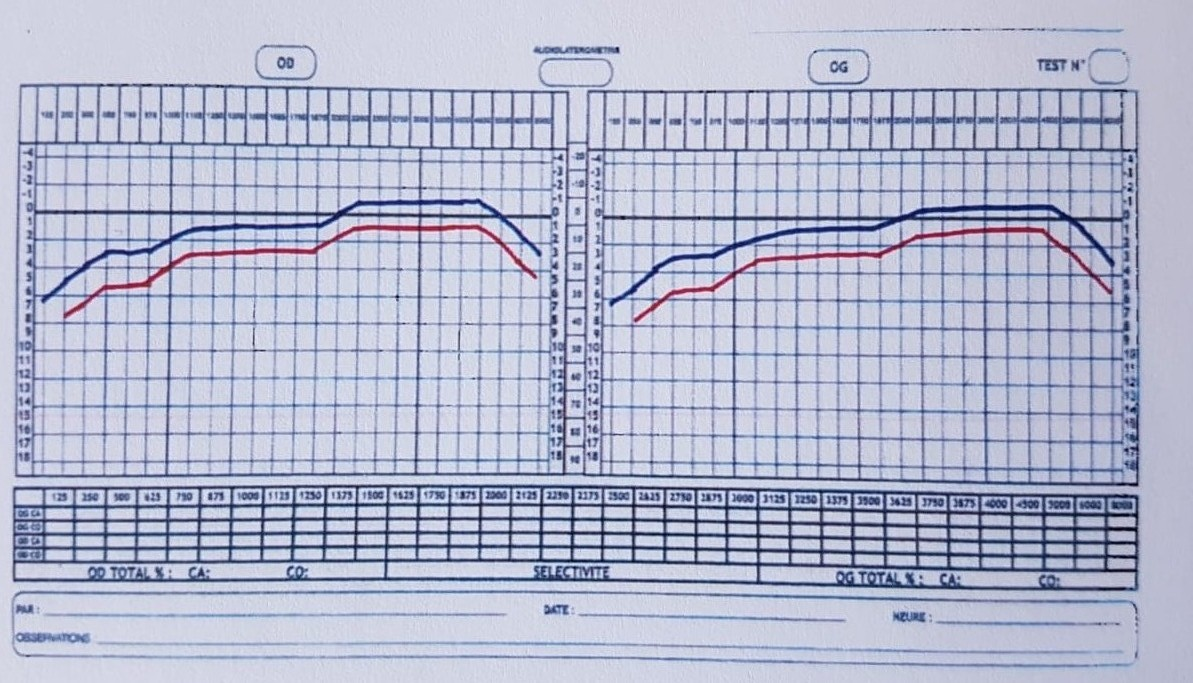
\includegraphics[width=0.7\linewidth]{images/courbeideale.jpg}
	\caption{Courbe idéale}
	\label{fig:courbeideale}
      \end{figure}

      
Sur le plan de la physique pure, elle indique les réponses de l'oreille
lorsque celle-ci fonctionne bien. Elle répond en fait à la courbe
de Wegel dite ``courbe en citron", inversée.\footnote{%
		Voir l'annexe \ref{acoustique} p. \pageref{acoustique}
		 pour cette partie technique.}.

               

L'acquisition de cette courbe idéale correspond à l'\textsl{harmonisation}
du jeu de deux muscles de l'oreille moyenne. Ce jeu
permet de régler en permanence la pression interne au niveau du
labyrinthe.
Lorsque l'interprétation des informations transmises à l'oreille est
erronée, il s'agit donc  de
distorsions d'écoute, déjà citées plus haut. Cette distorsion est liée au dysfonctionnement
de ces deux muscles de l'oreille moyenne dont le rôle est de permettre l'arrivée
harmonieuse du son dans l'oreille interne, puis au cerveau. Car, lorsque
le message sensoriel est altéré, le cerveau se protège en déclenchant
des mécanismes d'inhibition de l'écoute. On naît
avec ce potentiel mais celui-ci s'altère parfois avec les difficultés
de la vie et on introduit des distorsions
pour se défendre contre certaines agressions du monde extérieur. 

Sur le plan du test d'écoute, on remarquera
alors des distorsions, des manques par rapport à la courbe dite 
idéale.
Et lorsqu'il n'y a pas de distorsions, on parle d'harmonie. L'harmonie
est la régulation des émotions, l'équilibre entre son écoute
intérieure et extérieure. On la visualisera sous la forme de
courbes continues et parallèles.
Ces paramètres sont importants et nous reviendrons plus en détail sur le test d'écoute :(8.3.2)
%\enquote{\emph{L'oreille a un
%psychisme\autocite[{tomatis:loreille}.}} 




  




 




  

